\section{N2Sky Architecture}\label{TheN2SkyArchitecture}

\subsection{Current Architecture Analysis}\label{CurrentArchitectureAnalysis}
\subsubsection{Architecture design}\label{Architecturedesign}
\subsubsection{Components}\label{Components}
\subsubsection{Current User Interface}\label{CurrentUserInterface}
\subsubsection{Usability and user experience}\label{Usabilityanduserexperience}



\subsection{Redesign motivation}\label{Redesignmotivation}

Application redesign is a project, which takes a lot of work. But at some point every designer faced a refactoring project. It has a lot to do with user experience. Bad user experience will make users stop use an application and leave negative feedback on application in general. 

\subsubsection{Redesign Process }\label{Redesign Process}

There is data, information and user experience of previous version of N2Sky to work with. Making redesign it is already known who the users are and what they are trying to achieve.  Using this information it is possible to build an aims for a future user interface and user experience.


\begin{description}

\item[Finding problems.]  There are multiple problems with the application. One of the most crucial is that user interface is not intuitive understandable. 
\begin{figure}[htbp]
\begin{center}
  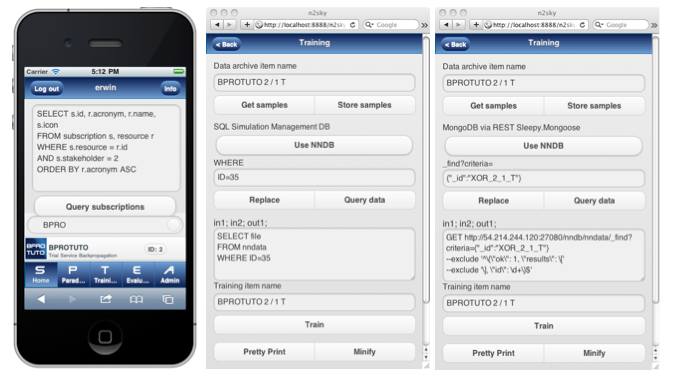
\includegraphics[width=\linewidth]{components/2/old_arch.png}
  \caption{Current N2Sky User Interface}
  \label{fig:old_arch}
\end{center}
\end{figure}


After signing in user getting subscription form, paradigm service and paradigm metadata views without any field description. Small titles unfortunately not always self-describing. Application in general oriented on the group of users, who are came from IT area. In some forms they can type queries, but the fields are not type safe and there is no autocomplete.
Representation of neural networks trained model is not readable. The model represented as a raw JSON or XML file, user can not download it. The last point is a design in general that does not look up-to-date and user attractive. 


\item[User interviews and Questionnaire.]
User insights are very important. It helps to understand a nature of the problem. But if user find something confusing, the interviewer need to dig deeper to stress the importance of particular insight. Unfortunately there were no analytics data and any reviews regarding UI and UX, so with a small group of colleges the current UI of N2Sky was reviewed. 
The following questions were derived (Q1-Q5): 


\begin{itemize}
\item Q1: "How N2Sky can help you with a developing of your neural network?"
\item Q2: "What was the most difficult part by creating a new model?"
\item Q3: "Did you face any problems during spawning your neural network? If yes, then what kind?"
\item Q4: "Did you find out something new, when other users were performing testing against your neural network?"
\item Q5: "What did you miss during using an N2Sky?"
\end{itemize}	

There were 5 students interviewed. All students were together in one group. Summarise answers (A1-A5) according to questions (Q1-Q5): 

\begin{itemize}
\item A1: N2Sky gives possibility to test the own neural network. Unfortunately, if the user does not have a neural network it is impossible to test the application.   
\item A2:  User face difficulties during creation of the new neural network model. User interface user technical jargon and it is not intuitively understandable.  
\item A3:  Spawning a neural network was pretty clear process, but it was not really clear if neural network ready to use or not.
\item A4:  Logging of the training data is very useful. The neural network owner can see how his network behaves with a different training and testing data.
\item A5:  User wants perform testing and training on already existing neural networks. 
\end{itemize}	


\item[Current application design mapping.]

After studying the answers it is possible to highlight weak parts of application. This approach will show a big picture of the current application design:

\begin{itemize}
\item Arbitrary user needs to know multiple technologies and programming languages just simply to reuse existing neural network. 
\item Too much information on every view. The purpose of view is overloaded. Each view has too much functionality, which makes user to loose a focus.
\item Application works relatively slow. Even if there some processes behind happening, the user des not know it.
\end{itemize}

Important is to face the problems, but does not "reinvent the wheel".  As \hl{Joel Spolsky the} founder of Netscape and CEO of Stack Overflow said, ??throwing away the whole program is a dangerous folly?. That is why it was decided to consider the problems of current N2Sky design and reuse working ideas in refactored system

\item[Application Maintenance.]
N2Sky was monolithic standalone application, which included all services in one and was deployed as a whole. The application was not distributed.  In case if one of the services doesn?t work correct, the whole application is not usable. 
Originally the previous version of N2Sky was written fully on Java. There were hundreds classes, providers and services in one project. Developer will spend hours to maintain this kind of project. To find an issue in a big application is always a challenge.  Small changes are causes a subsequence changes. If the software breaks after change, than it will additional high effort to fixed it. As Robert Cecil Martin wrote in his book ?Clean Code?: ?The code is hard to understand. Therefore, any change takes additional time to first reengineer the code and is more likely to result in defects due to not understanding the side effects? \hl{[https://www.amazon.com/Clean-Code-Handbook-Software-Craftsmanship/dp/0132350882]}.  He categorizes this kind of code into ?Smell? code. Unfortunately N2Sky from maintain perspective had all problems, which Mr. Martin

That is why N2Sky is shifted from monolithic system to container based system with an independent micro services which located on cloud environment. 
The frontend and frontend services are lightweight and easy to maintain parts of the big application. If something goes wrong, the developer knows exactly where is the problem. It is close to impossible to break something else during fixing because of independence of services. 
Additionally there are monitoring and alerting systems which are supporting developers during maintenance.  Early it was not possible to say if application works correctly or even it still running. Users could get a bad experience while they using an application in case if it does not work correctly. But now it is possible not only notify an application administrator about some problems, but also to predict potential threads. 
\end{description}


\subsubsection{Refactoring the User Interface}\label{Refactoring the User Interface}

User Interface (UI), an abbreviation of user interface, allows the interaction of a user with a program through graphical visualization made by text, icons, buttons and pictures. While deciding the design of a user interface there are some highly recommended features also known as heuristics, which was invented by hl{Jakob Nielsen}. It was decided to apply the following 10 general principals of interaction design to N2Sky:

\begin{description}
\item[Simple and natural dialogue.]  N2Sky will have an simple UI which is understandable for any user, even if the user is not an expert. Every icon and every navigation or action button will be self-describing. The application will follow the slogan ?less is more?. No more overloaded views. The idea of N2Sky UI design is that one particular view is responsible for one particular function or group of functions which a coupled tight together.
\item[Speak the users language.] Developing N2Sky was concentrated on user perspective. There is no technical jargon for arbitrary user.
\item[Minimize user memory load.] There is no multiple options, functions or menus on one view. There is also no multiple ways to do the same thing. N2Sky teach user how to make things done with a one existing and convenient workflow. 
\item[Consistency.] N2Sky has similar layouts, fonts, colors, icons types structures and organization throw entire application. The user should get the same visual experience on every view.
\item[Feedback.] Every action, process or even error will be notified. User will know exactly what is happening with a system with clear and understandable messages.
\item[Clearly marked exits.]  Every push to action button has short and clear caption.
\item[Shortcuts.] N2Sky has multiple user types. One of the types is the expert users, which are advanced user in neural network and artificial intelligence topics. For this kind of user is provided more technical jargon, but this UI is separated with an arbitrary users.  
\item[Good error messages.] Every notification is clear inclusive an error massage if occurs. Every message has a prices and simple description.
\item[Prevent errors.] In N2Sky implemented logical structure of UI components. There are constrains which are helps user in workflow. For example user will always get a default value of any input.
\item[Help and documentation.] N2Sky will have tutorials that describe the user workflow. The expert users will also get a API documentation with a detailed description and sample requests. 

\end{description}

Each and every one of these heuristics is connected to a crucial idea that is usability. By mentioning this idea, a straightforward relation with the UX follows since this is also one of the key concept that grows along the rapid development of technology. UX is known as user experience and it describes the perspective and feelings a user gets when interacting with product. It deepens into such aspect as the users inner circumstances and the nature of the created design. The goal is to achieve such a system that offers distinguished user experience and accomplishes the most of aspects. As above mentioned, usability.  \hl{(1)}
Putting both of UI and UX in a comparison, to all appearances the user interface is the target on the appearance and functionality of the product and its tangible details.  Furthermore, the user experience is the general experience that the user manages throughout the whole use.   \hl{(2)}
UI will concentrate on the appearance and design of the product, rather than the functionality. The intent of it relies in the visual design and layout. UI covers issues such as how a button is supposed to look like, how the errors are going to appear or is it visually comprehensible meaning which colors or font type shall be used for a better perceptibility of the product.  \hl{(6)}
UX points its focus on the involvement of the user while interacting. It is measured by a variety of tests and researches done to achieve a higher satisfaction on the users side.  \hl{(4)}
Though their differences, the only matter which relates both UI and UX is their priority, in other words, the user. When expanding the concept of both these definitions it can be concluded that one co-exists with the other. There would not be user interface without user experience and vice versa. 

 \hl{TODO // CHECK MERSI DOKU}

\subsubsection{Introducing a new User Experience Design}\label{Introducing a new User Experience Design}

 \hl{TODO}


\subsection{Contemporary N2Sky Architecture}\label{Contemporary N2Sky Architecture}

The user-centered design is a fundamental requirement for N2Sky. Looking back on past experiences with the application, there were identified the real capabilities and needs of a users. N2Sky was moved from a complex monolithic system to an easy understandable application. Every interested user without having a deep knowledge in the neural network field can freely use N2Sky.  The goal was to save and gain the current functionality of the application and decrease the visual complexity of it. 

\subsubsection{Architecture design}

N2Sky is a simulation platform, which allows all involved stockholders to use it for computational purposes. In order to achieve high performance and scalability, it was decided to use the microservices architecture. This approach is used not only on backend services, but also with frontend and its services. 

\begin{figure}[htbp]
\begin{center}
  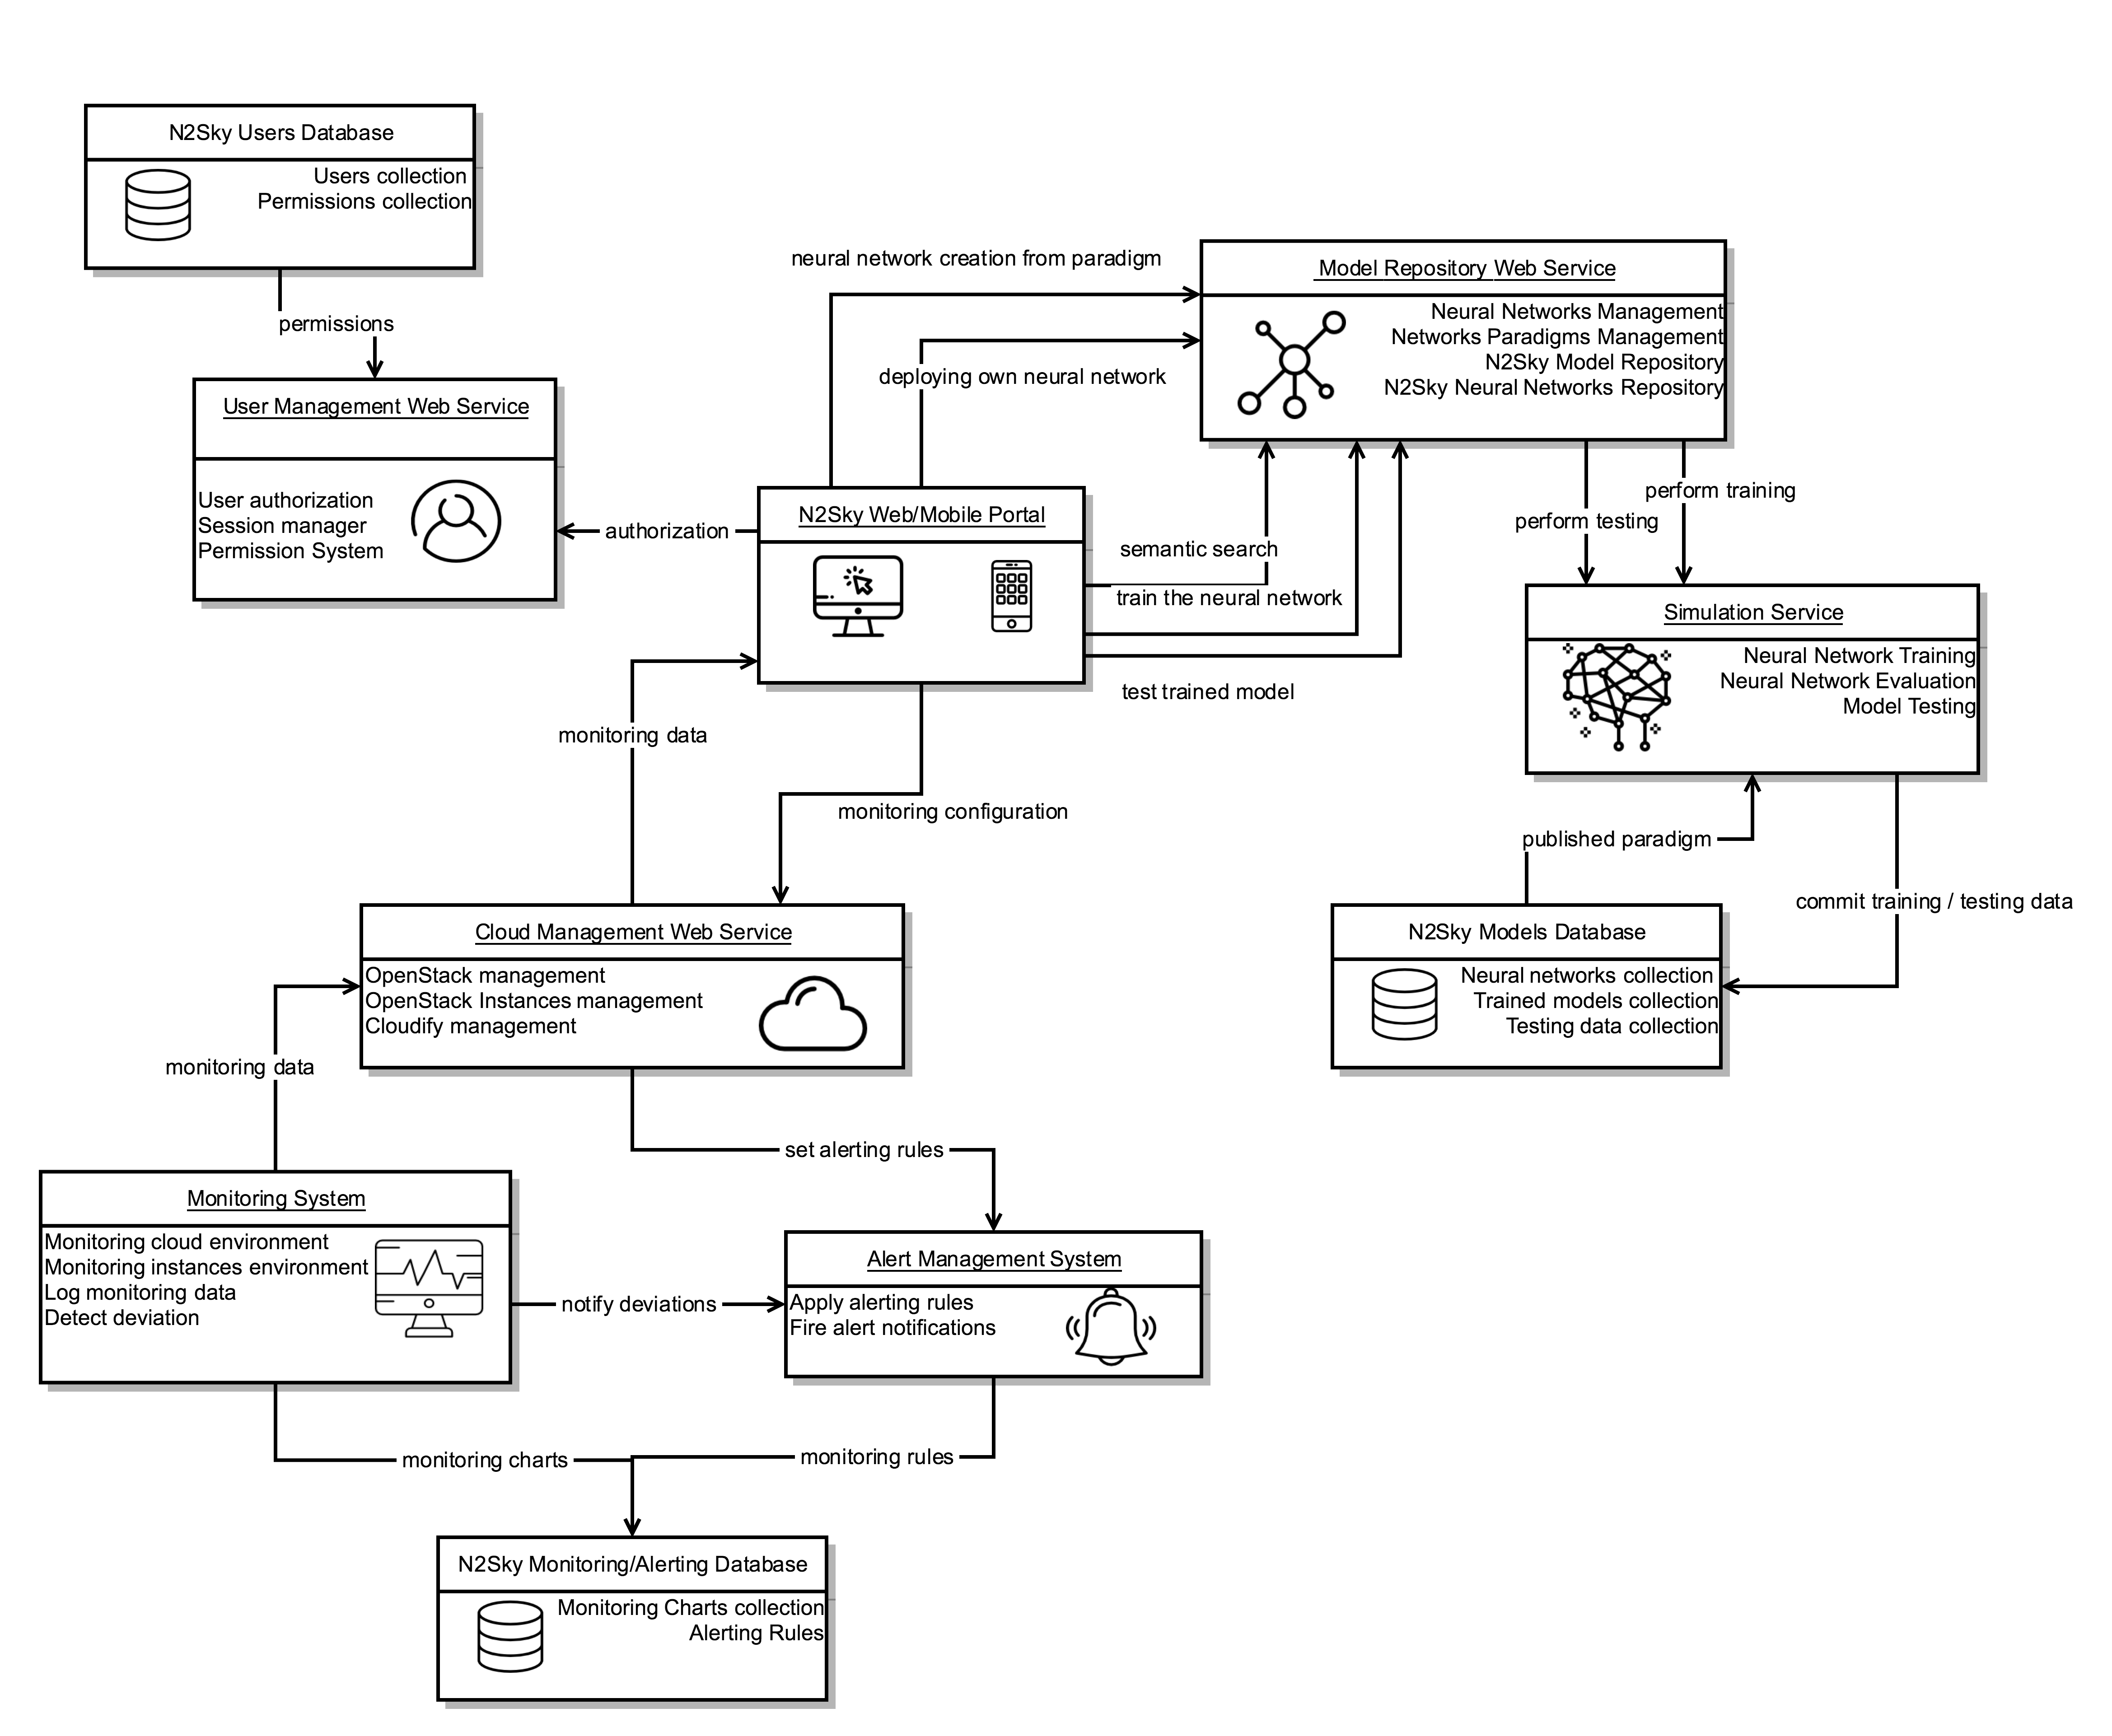
\includegraphics[width=\linewidth]{components/2/new_arch.png}
  \caption{Contemporary N2Sky architecture overview}
  \label{fig:newarch}
\end{center}
\end{figure}

The architecture overview, which shown in ``Fig.~\ref{fig:newarch}'' represents microservices architecture. 

The centred figure is the N2Sky Web/Mobile portal. Is is frontend application of the N2Sky, which consist of modular subsystems. Since the frontend application has responsive design it supports desktop devices as well as mobile devices. 
To support Software as a Service distribution every web service can work independently. It means that the stackholders can use N2Sky via web portal as well as use N2Sky API.
N2Sky API allows  stackholders:

\begin{itemize}
\item Authorise in the System
\item Create new neural from existing paradigm
\item Deploy own neural network on N2Sky environment 
\item Perform training against own as well published neural network
\item Perform testing against trained models
\end{itemize}

Almost everything is available for arbitrary stackholder, except cloud services. In order to cloud service as a service, the user has to install it on his own cloud environment. This approach supports Platform as a Service distribution. Cloud services only for system administrator and for granted users are available. 


\subsubsection{N2Sky Services}\label{N2Sky Services}

 N2Sky implements microservices architecture. It has 3 main web services as it shown in ``Fig.~\ref{fig:newarch}'' :
 
\begin{itemize}
\item User Management Web Service
\item Model Repository Web Service
\item Cloud management Web Service
\end{itemize}

Every web service use other services which are not exposed to the public. It was made in order to support application encapsulation. Encapsulation of web application helps to prevent security issue. One of the crucial crucial process in N2Sky is the neural network training. This process takes almost all resources of the environment, that is why it is not exposed. Such a processes can be triggered only by web service, which can be blocked if environment is overloaded.

Consider the following web services in details and which processes and services they are encupsulate:  

\begin{description}
\item[User Management Web Service.]   This web service responsible for permissions and user management and it has its own database. User can authorise in the system and get a session token. Every token is an unique collection of numbers and latin letters. Token is assign to the authorised user and will be save until user is active. If user is not active in the next 3 hours, the session token will disappear. If user still have an active browser session, the authorisation token will be revalidate. If user trying to make some illegal request or behave too active, the authorisation token will be revoked and the system administrator will be notified about this incident. 

Every user encapsulate permission level. There two different types of permissions:
\begin{itemize}
\item Administrator permission. It means, that the user has full granted permission throw entire application.
\item Regular permission. The user has access only for his own as well as public available resources.  
\end{itemize}
\item[Model Repository Web Service.]  Model Repository Web Service is the core service of N2Sky. Authorised user can create a new project, add there neural network from chose paradigm or deploy own one. Every newly created project is assign for one user and can not be shared, only system administrator can look up into other users projects. This functionality also limited by User Management Web Service. 

Using this service user can create a neural network from proposed paradigms as well as upload his own neural network in \hl{ViNNSL} format. This functionality exposed via service so that every user can use it either from N2Sky web portal or via HTTP request directly on web service.

There are two services embedded to the Model Repository web service and not exposed:

\begin{description}
\item[Training service.]  This service provides neural network training functionality. It is not possible to perform training to make direct request on service endpoint. 

In order  to perform training the user has to know training input parameters and type of training file which ca be accepted. This information is stored in ViNNSL schema. 
 
Only Model Repository web service can trigger this service after being insured that environment available and ready to perform tests. Training a is long term process, but it does not block an entire application. This service write log data to the instance. Model Repository repository makes a callback to training service in order to check if training is completed. If training still processing, the Model Repository Service will fetch the log data in order to present current training result. User can also decide to stop training process if he is satisfied with the current result.

If user perform training on his own neural network he can also log result about his network and enviroment behaviour. 
\item[Testing service.] The testing service allows users to evaluate a trained model.  Testing data is described in ViNNSL format. Normally testing is not a long term process, because it is running agains trained neural network model. Since there is absolute freedom by neural network structure customisation, the testing process can be inefficient and could take some resources from the environment. Considering this face it was decided to encapsulate this process too. 
\end{description}

 \item[Cloud management Web Service.]  Cloud web service is originally available only for system administrator. This service can manage OpenStack environment and Cloudify container management system. On every OpenStack instance as we as on OpenStack itself the monitoring management system service is installed. Every monitoring management system has its own metrics configurations and alerting rules. The monitoring service is only exposed via Cloud management web service. 
 
 Cloud management service supports Platform as a Service distribution. The system administrator can configure the service according to his needs. All rules, including configuration rules for monitoring and alert management systems, can be adjusted on demand.  


\end{description}



 
 
\subsubsection{Modular frontend application design}
The central concept of the application is to support the \hl{Software as a Service (SaaS)} and Platform as a Service (PaaS) distributions.  N2Sky consist of two modules: administration module, main application module as it shown in ``Fig.~\ref{fig:modular_design}''.

\begin{figure}[htbp]
\begin{center}
  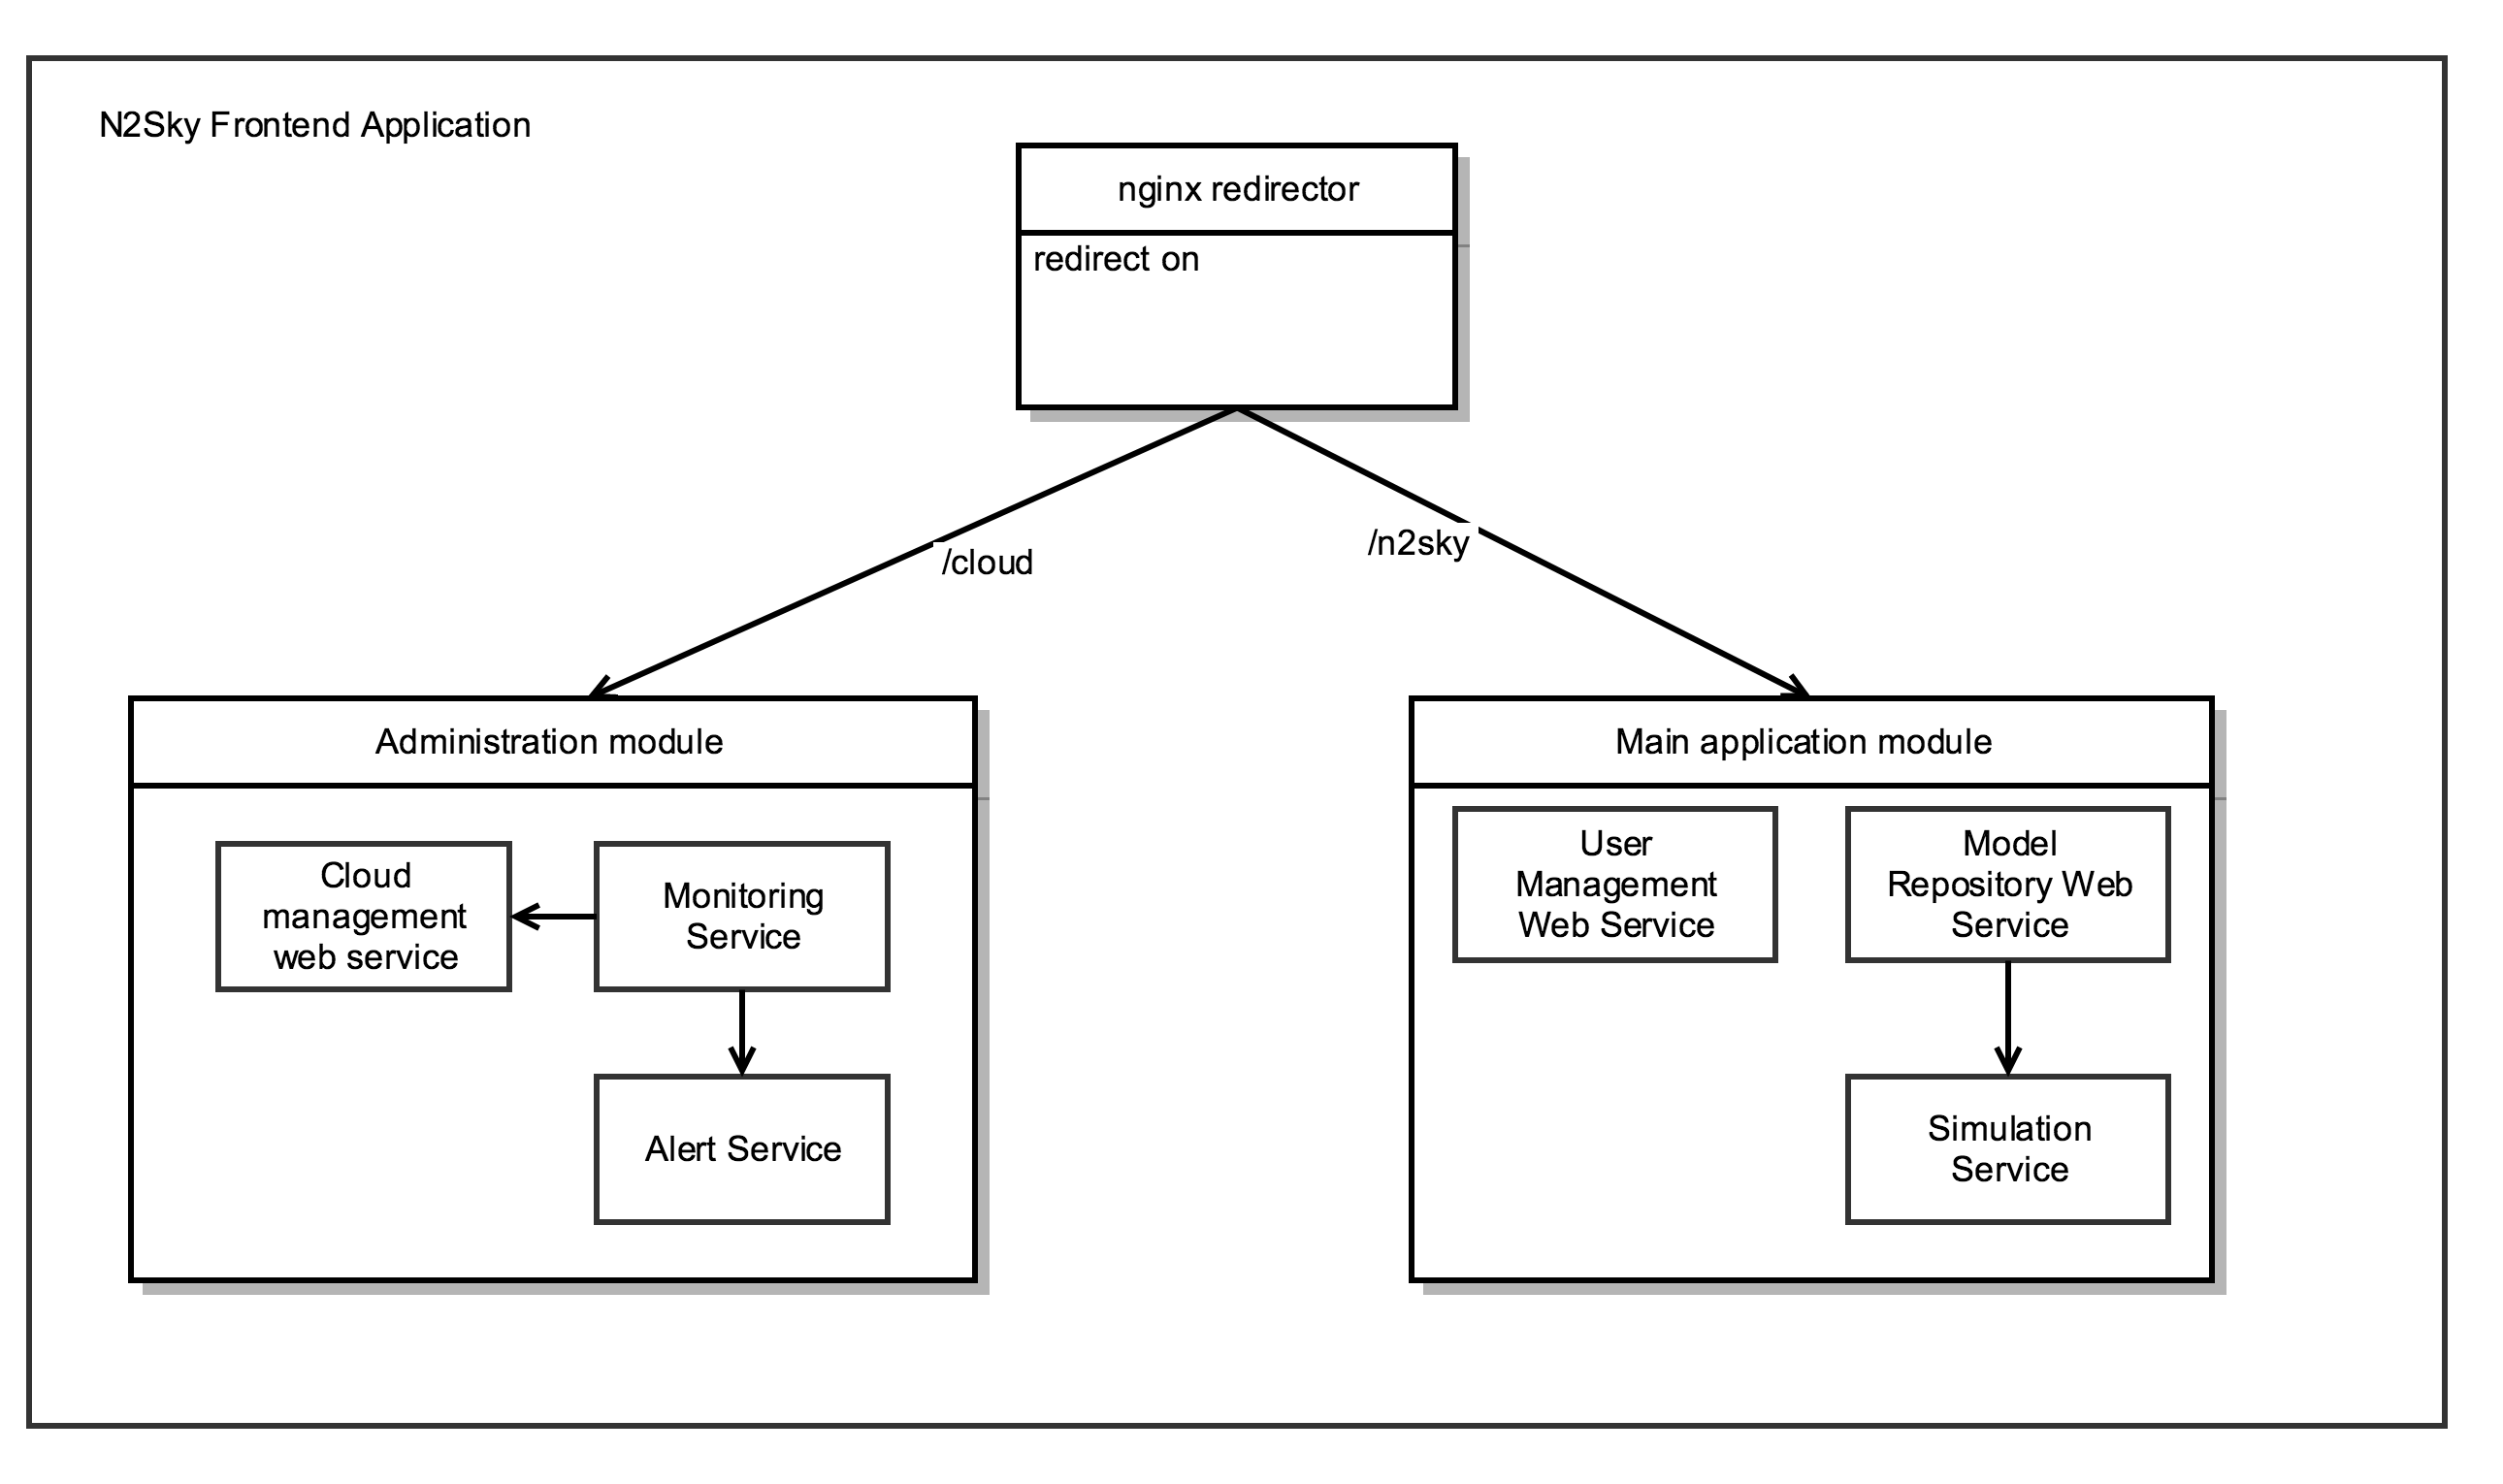
\includegraphics[width=\linewidth]{components/2/modular_design.png}
  \caption{N2Sky frontend application and its services}
  \label{fig:modular_design}
\end{center}
\end{figure}

\begin{description}
\item[Redirector.] When the user goes to N2Sky web portal, first he will be dealing with a redirector. The redirector is a small service, which is build on Nginix server. The purpose of it is to redirect the user depending on URL path.
\begin{description}
\item[/cloud] redirects to "Administration module"
\item[/n2sky] redirects to "Main application module"
\end{description}


\item[Administration module] The administration module allows the system administrator to control the environment. The module supports OpenStack and Cloudify monitoring. Managing is possible through the application dashboard. It also contains custom monitoring and an alerting management system, which can be installed on any server within the N2Sky user interface. The administration module implements PaaS. It is fully configurable and wrapped into the open source project in order to make the module accessible to the third-party applications. 
\item[Main application module] The main application module is the central module of N2Sky. Within this module, users can use, train and test existing neural networks. It is possible to reuse the neural network paradigms and create own neural network. N2Sky allows to deploy own network and store data in cloud. Module services are supporting the SaaS distribution. Experts can use an application directly through the N2Sky API or they can integrate N2Sky services to their own application. 
\end{description}


 

\subsubsection{Technology Stack}\label{Technology Stack}

N2Sky today is the cross-platform handy application with a responsive design. Create own framework from scratch would be time consuming. To build cross-platform framework just for N2Sky is an absurd. After some research of most popular and common used frontend frameworks following candidates were listed: 

\begin{description}
\item[Vaadin.] Java framework, which compiles Java code into JavaScript components. Vaadin supports cross-platform application, but not fully. It is possible to wrap an applicaiton into container and deploy it only as an android application.

\begin{description}
\item[Benefits.] Easy to develop in Java. Developer does not have to think about JavaScript functionality. There are dozen of predefined components like: buttons, input fields, frames etc. Customisation is also possible. 
\item[Obstructions.] Deployment process is a blockage process. There is no "hot redeployment" available. Even if developer win some time by build components in Java, he will lose much more time by continuous redeployment. 

Java application need some server which supports JVM, it means that server should have much more memory then some other frameworks, which are written on JavaScript language.  
\end{description}

\item[ReactJS.]  JavaScript framework, which supports JSX programming language. 
\begin{description} 
\item[Benefits.] The main idea is to write HTML code in JavaScript. ReactJS supports hot redeployment.  React-Native extension for this framework, which allows to wrap the whole application mobile as well as desktop application.
\item[Obstructions.]  Difficult to support a big project. JSX is not a type safe programming language. Exception handling also need to be done by developer.  
\end{description}
\item[AngularJS.] JavaScript framework, which supports TypeScript programming language.
\begin{description} 
\item[Benefits.] The main idea is to write JavaScript code in HTML.  AngularJS same as ReactJS supports hot redeployment.  It does not have native support for all mobile devices, but is possible to wrap it using IONIC framework. 
\item[Obstructions.]  AngularJS compiles TypeScript code into JavaScript core and sometimes compilation fails because TypeScript is a new language and it is not fully adopted for browsers. 
\end{description}
\end{description}
 
 Vaadin does not fit N2Sky needs, but AngularJS and ReactJS could fit perfectly. Both of this frameworks are written on JavaScript and have big corporations behind: AngularJS was developed by Google and ReactJS was developed by Facebook. Since N2Sky has to support fully cross-platform architecture it was decided to choose ReactJS. With this framework N2Sky has a potential to be multi-platform application in the future. 
 

Furthermore, backend has microservices architecture to support scalability. After choosing JavaScript framework for frontend it will make sense to user JavaScript in a backend too, so that server would be small and fast. Each one of the microservices is developed on NodeJS Framework server, which implies efficiency and lightweight. 

N2Sky is a cloud-based system. OpenStack cloud platform supports this approach. Since N2Sky user OpenStack API for administration dashboard, the original OpenStack dashboard was no more needed. Every backend and frontend service is deployed on OpenStack instance. Every instance is absolutely scalable, which allows to find a best enviroment for every service. 

Every OpenStack instance is a server with either Debian or Ubuntu operational system. Every instance as well as OpenStack itself has to be monitored 24/7, that is why there was Monitoring Management System developed. The basis of this system is Prometheus monitoring system, which gives full access to all information of any server were its was installed. Prometheus has an open API, which is used by N2Sky. Using Prometheus there were charts and graphs developed and integrated into N2Sky. Alert Management System, which is a part of N2Sky, is also using  Prometheus API in order to detect deviation and notify on event occurred.

As a database it was decided to choose NoSQL one. There were two NoSQL databases under consideration ElasticSearch and MongoDB. 
ElasticSearch supports indexes. It is possible to configure index so, that is impossible to insert something which is not mapped by the index.  MongoDB does not user index approach, but MongoDB client supports schema. It was decided to use MongoDB schema and mapped ViNNSL schema to it in order to make it more understandable for other developers. 

For continuous delivery and quick configuration it was decided to use Jenkins Continuous Integration system. In case if the while system will go down it is possible to restore every service with a Jenkins Profiles.


